% !TEX TS-program = pdflatex
% !TEX encoding = UTF-8 Unicode

% This is a simple template for a LaTeX document using the "article" class.
% See "book", "report", "letter" for other types of document.

\documentclass[11pt]{article} % use larger type; default would be 10pt

\usepackage[utf8]{inputenc} % set input encoding (not needed with XeLaTeX)

%%% Examples of Article customizations
% These packages are optional, depending whether you want the features they provide.
% See the LaTeX Companion or other references for full information.

%%% PAGE DIMENSIONS
\usepackage[a4paper,left=1.5cm,right=1.5cm,top=1.5cm,bottom=1.5cm]{geometry}
%\usepackage{geometry} % to change the page dimensions
% \geometry{a4paper} % or letterpaper (US) or a5paper or....
% \geometry{margin=0in} % for example, change the margins to 2 inches all round
% \geometry{landscape} % set up the page for landscape
%   read geometry.pdf for detailed page layout information

\usepackage{graphicx} % support the \includegraphics command and options

\usepackage[parfill]{parskip} % Activate to begin paragraphs with an empty line rather than an indent

%%% PACKAGES
\usepackage{booktabs} % for much better looking tables
\usepackage{array} % for better arrays (eg matrices) in maths
\usepackage{paralist} % very flexible & customisable lists (eg. enumerate/itemize, etc.)
\usepackage{verbatim} % adds environment for commenting out blocks of text & for better verbatim
\usepackage{subfig} % make it possible to include more than one captioned figure/table in a single float
\usepackage{amsmath}
\usepackage{amssymb}
\usepackage{logicproof}
\usepackage{tikz}
\usetikzlibrary{arrows,petri,topaths}
\usepackage{float}
\usepackage{multicol}
\setlength{\columnsep}{-3cm}
% These packages are all incorporated in the memoir class to one degree or another...

%%% HEADERS & FOOTERS
\usepackage{fancyhdr} % This should be set AFTER setting up the page geometry
\pagestyle{fancy} % options: empty , plain , fancy
\renewcommand{\headrulewidth}{0pt} % customise the layout...
\lhead{}\chead{}\rhead{}
\lfoot{}\cfoot{}\rfoot{}

%%% SECTION TITLE APPEARANCE
\usepackage{sectsty}
\allsectionsfont{\sffamily\mdseries\upshape} % (See the fntguide.pdf for font help)
% (This matches ConTeXt defaults)

%%% ToC (table of contents) APPEARANCE
\usepackage[nottoc,notlof,notlot]{tocbibind} % Put the bibliography in the ToC
\usepackage[titles,subfigure]{tocloft} % Alter the style of the Table of Contents
\renewcommand{\cftsecfont}{\rmfamily\mdseries\upshape}
\renewcommand{\cftsecpagefont}{\rmfamily\mdseries\upshape} % No bold!
\renewcommand{\thesection}{}
\renewcommand{\thesubsection}{Iteration \arabic{subsection}}
\newcommand{\qedsymbol}{\rightline{$\blacksquare$}}
\newcommand{\selected}[1]{\textcolor{teal}{\textbf{#1}}}


%%% END Article customizations

%%% The "real" document content comes below...

\title{MCS Assignment}
\author{zrlr73}
%\date{} % Activate to display a given date or no date (if empty),
         % otherwise the current date is printed 

\begin{document}
\section{\textbf{Question 2} \hfill zrlr73}




\subsection{}
\begin{multicols}{2}
\begin{tabular}{c|c c c c c c|}
	 & a & b & c & d & e & f \\
	\hline
	a & 0 & \selected{15} & 24 & 29 & 25 & 37 \\
	b && 0 & 32 & 31 & 23 & 43 \\
	c &&& 0 & 30 & 43 & 49 \\
	d &&&& 0 & 45 & 57 \\
	e &&&&& 0 & 55 \\
	f &&&&&& 0 \\
	\hline
\end{tabular}

\columnbreak

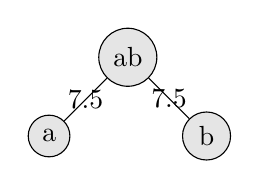
\begin{tikzpicture}[main_node/.style={circle,fill=gray!20,draw,minimum size=1em,inner sep=3pt}]
	\node[main_node] (a) at (0,0) {a};
	\node[main_node] (b) at (2,0) {b};
	\node[main_node] (ab) at (1,1) {ab};
	
	\draw{(a) edge node {7.5} (ab)};
	\draw{(b) edge node {7.5} (ab)};
\end{tikzpicture}
\end{multicols}




\subsection{}
\begin{multicols}{2}
\begin{tabular}{c|c c c c c|}
	 & c & d & e & f & ab \\
	\hline
	c & 0 & 30 & 43 & 49 & 28 \\
	d && 0 & 45 & 57 & 30 \\
	e &&& 0 & 55 & \selected{24} \\
	f &&&& 0 & 40 \\
	ab &&&&& 0 \\
	\hline
\end{tabular}

\columnbreak

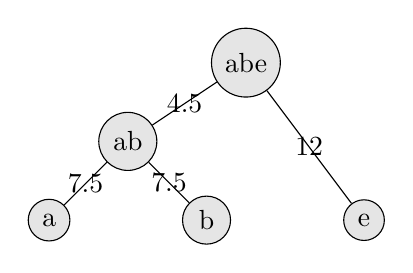
\begin{tikzpicture}[main_node/.style={circle,fill=gray!20,draw,minimum size=1em,inner sep=3pt}]
	\node[main_node] (a) at (0,0) {a};
	\node[main_node] (b) at (2,0) {b};
	\node[main_node] (ab) at (1,1) {ab};
	\node[main_node] (e) at (4,0) {e};
	\node[main_node] (abe) at (2.5, 2) {abe};
	
	\draw{(a) edge node {7.5} (ab)};
	\draw{(b) edge node {7.5} (ab)};
	\draw{(e) edge node {12} (abe)};
	\draw{(ab) edge node {4.5} (abe)};
\end{tikzpicture}
\end{multicols}




\subsection{}
\begin{multicols}{2}
\begin{tabular}{c|c c c c|}
	 & c & d & f & abe \\
	\hline
	c & 0 & \selected{30} & 49 & 33 \\
	d && 0 & 57  & 35 \\
	f &&& 0 & 45\\
	abe &&&& 0 \\
	\hline
\end{tabular}

\columnbreak

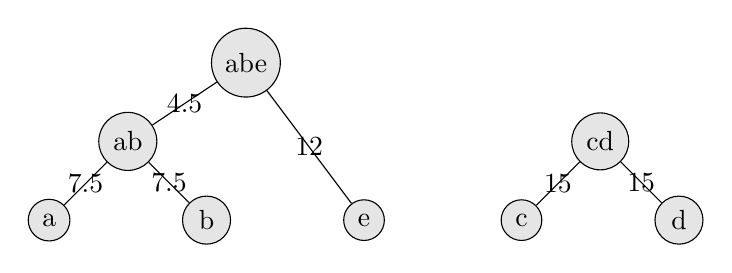
\begin{tikzpicture}[main_node/.style={circle,fill=gray!20,draw,minimum size=1em,inner sep=3pt}]
	\node[main_node] (a) at (0,0) {a};
	\node[main_node] (b) at (2,0) {b};
	\node[main_node] (ab) at (1,1) {ab};
	\node[main_node] (e) at (4,0) {e};
	\node[main_node] (abe) at (2.5, 2) {abe};
	\node[main_node] (c) at (6, 0) {c};
	\node[main_node] (d) at (8, 0) {d};
	\node[main_node] (cd) at (7, 1) {cd};
	
	\draw{(a) edge node {7.5} (ab)};
	\draw{(b) edge node {7.5} (ab)};
	\draw{(e) edge node {12} (abe)};
	\draw{(ab) edge node {4.5} (abe)};
	\draw{(c) edge node {15} (cd)};
	\draw{(d) edge node {15} (cd)};
\end{tikzpicture}
\end{multicols}




\subsection{}
\begin{multicols}{2}
\begin{tabular}{c|c c c|}
	 & f & abe & cd \\
	\hline
	f & 0 & 45 & 53 \\
	abe && 0 & \selected{34} \\
	cd &&& 0 \\
	\hline
\end{tabular}

\columnbreak

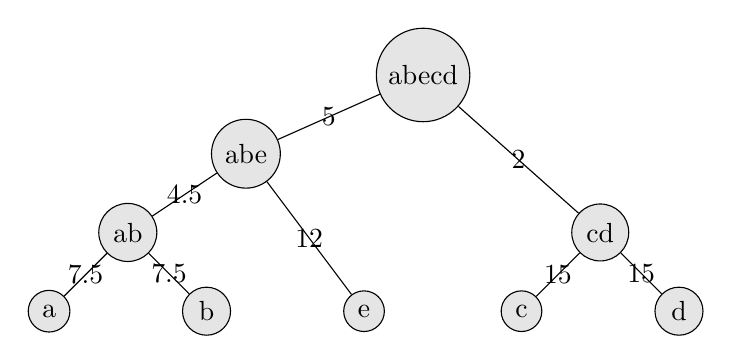
\begin{tikzpicture}[main_node/.style={circle,fill=gray!20,draw,minimum size=1em,inner sep=3pt}]
	\node[main_node] (a) at (0,0) {a};
	\node[main_node] (b) at (2,0) {b};
	\node[main_node] (ab) at (1,1) {ab};
	\node[main_node] (e) at (4,0) {e};
	\node[main_node] (abe) at (2.5, 2) {abe};
	\node[main_node] (c) at (6, 0) {c};
	\node[main_node] (d) at (8, 0) {d};
	\node[main_node] (cd) at (7, 1) {cd};
	\node[main_node] (abecd) at (4.75, 3) {abecd};
	
	\draw{(a) edge node {7.5} (ab)};
	\draw{(b) edge node {7.5} (ab)};
	\draw{(e) edge node {12} (abe)};
	\draw{(ab) edge node {4.5} (abe)};
	\draw{(c) edge node {15} (cd)};
	\draw{(d) edge node {15} (cd)};
	\draw {(abe) edge node {5} (abecd)};
	\draw {(cd) edge node {2} (abecd)};
\end{tikzpicture}
\end{multicols}




\subsection{}
\begin{multicols}{2}
\begin{tabular}{c|c c|}
	 & f & abecd \\
	\hline
	f & 0 & \selected{48.2} \\
	abecd && 0 \\
	\hline
\end{tabular}

\columnbreak

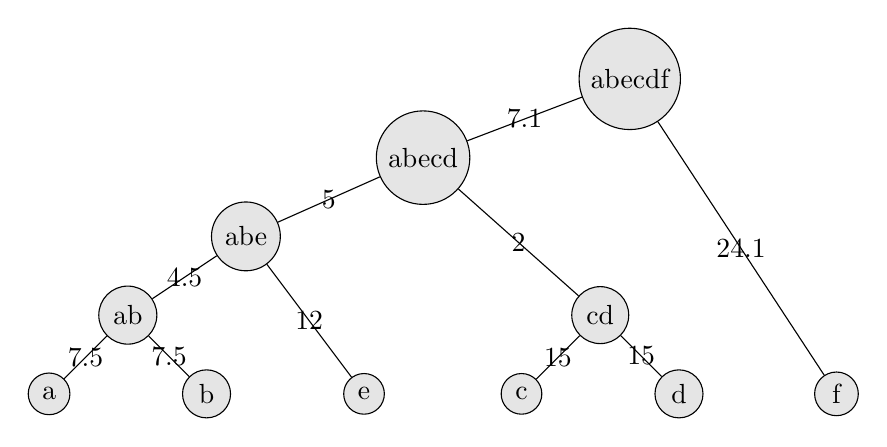
\begin{tikzpicture}[main_node/.style={circle,fill=gray!20,draw,minimum size=1em,inner sep=3pt}]
	\node[main_node] (a) at (0,0) {a};
	\node[main_node] (b) at (2,0) {b};
	\node[main_node] (ab) at (1,1) {ab};
	\node[main_node] (e) at (4,0) {e};
	\node[main_node] (abe) at (2.5, 2) {abe};
	\node[main_node] (c) at (6, 0) {c};
	\node[main_node] (d) at (8, 0) {d};
	\node[main_node] (cd) at (7, 1) {cd};
	\node[main_node] (abecd) at (4.75, 3) {abecd};
	\node[main_node] (f) at (10, 0) {f};
	\node[main_node] (abecdf) at (7.375, 4) {abecdf};
	
	\draw{(a) edge node {7.5} (ab)};
	\draw{(b) edge node {7.5} (ab)};
	\draw{(e) edge node {12} (abe)};
	\draw{(ab) edge node {4.5} (abe)};
	\draw{(c) edge node {15} (cd)};
	\draw{(d) edge node {15} (cd)};
	\draw {(abe) edge node {5} (abecd)};
	\draw {(cd) edge node {2} (abecd)};
	\draw {(f) edge node {24.1} (abecdf)};
	\draw {(abecd) edge node {7.1} (abecdf)};
\end{tikzpicture}
\end{multicols}

\end{document}
